\graphicspath{{detail_design/fig/}}

\chapter{Detailed Design}
\label{chap:detail_design}

According to the electrical characteristics of the major components (shown in table \ref{tab:electrical_chars}), the entire system can be powered by a 6V source. A voltage regulator will be used to provide 5V to the microcontroller.
\\


\begin{table}[!h]
\centering
\caption{Electrical characteristics of major components.}
\label{tab:electrical_chars}
    \begin{tabular}{|c||c|c||c|c|} 
        \hline
        Component & \multicolumn{2}{c||}{Input} & \multicolumn{2}{c|}{Output} \\
       %\hline
         & Voltage [V] & Current [mA] & Voltage [V] & Current [mA] \\
        \hline
        \hline
        ESP32 \cite{esp_datasheet} & 3.3 & 500 & & \\
         & 5 & & & \\
        \hline
        ESP32 pins \cite{esp_datasheet} & 0.75 * $V_{DD}$ & & 0.8 * $V_{DD}$ & 40\\
        & $V_{DD}$ + 0.3 & & & \\
        \hline
        Soil moisture sensor \cite{Moisture_sensor_datasheet} & 3.3 & $< 5$ \tablefootnote{Based off measurements} & 1.2 (high moisture) & \\
        & 5.5 & & 2.5 (low moisture) & \\
        \hline
        UV light sensor \cite{UV_sensor_datasheet} & 3 & 100 \tablefootnote{Maximum rating based off characteristics of similar sensors} & 0 & \\
        & 5 & & 3 & \\
        \hline
        Pump \cite{pump_datasheet} & 6 & 1800 (2500 peak) \cite{pump_datasheet_similar} \tablefootnote{Based off characteristics of similar pump} & & \\
        \hline
    \end{tabular}
\end{table}
%%%%%%%%%%%%%%%%%%%%%%%%%%%%%%%%%%%%%%%%
\section{UV light exposure and soil moisture level measurement and logging}

The microcontroller uses a 5V supply to maximize the voltage output of the pins (this will make designing the pump driver circuit easier - the driver circuit is going to need like 7+ volts)
\\


Both the soil moisture and UV light sensors are designed to be powered by a microcontroller. Both sensors will therefore be powered using the 3.3V output pin on the ESP32. 
\\
Pins 2 and 3 (corresponding with ADC channels 2 and 3) will be used for the soil moisture and UV light sensor respectively

The default ADC measurement range of the ESP32-C6 is 0V to 1V \cite{esp_datasheet} \cite{esp_github}. The signals from the sensors must therefore be attenuated before being input to the ADC. The minimum attenuation as calculated in equation \ref{eqn:attenuation} \cite{attenuation_formula} is \(-10.37 dB\).

\begin{equation}
\label{eqn:attenuation}
\begin{split}
    Attenuation  (dB) & = 20 \cdot log_{10}\left ( \frac{V_{out}}{V_{in}} \right ) \\ 
    & = 20 \cdot log_{10}\left ( \frac{1}{3.3} \right ) \\ 
    & = -10.37 dB
\end{split}
\end{equation}

An attenuation of 11dB was used as it is the closest value provided by the ESP32 Arduino Core library \cite{esp_arduino_github} (which allows writing code for the ESP32-C6 using the Arduino IDE). 
\\
The ESP32-C6 has a 12 bit ADC \cite{esp_tech_ref}, resulting in a resolution of 4095, the sensor output ranges can be calculated using equation \ref{eqn:measured_val}. Table \ref{tab:sensor_ranges} shows the calculated measurement ranges of both sensors.

\begin{equation}
\label{eqn:measured_val}
    Measured \quad value = Resolution \cdot V_{in} \cdot 10^{Attenuation / 20}
\end{equation}

\begin{table}[!h]
    \centering
    \begin{tabular}{|c|cc|cc|}
    \hline
         & \multicolumn{2}{c||}{Soil moisture sensor} & \multicolumn{2}{c|}{UV light sensor} \\
        \hline
        Voltage & 1.2V & 2.5V & 0V & 3V \\
        Measured value & 1385 & 2885 & 0 & 3462\\
        \hline
    \end{tabular}
    \caption{Sensor value ranges}
    \label{tab:sensor_ranges}
\end{table}

%%%%%%%%%%%%%%%%%%%%%%%%%%%%%%%%%%%%%%%%
\section{Automatic watering}
The pump requires 6V and has a peak current of approximately 2.5A and a rated power of 5W (based on the rating of a similar pump). To accommodate the maximum potential power draw of 15W, a TIP31C npn power transistor will be used alongside a 2N2222A npn transistor in a Darlington pair. 
\\
The TIP31C has a maximum rated collector current of 3A and can dissipate up to 40W. The operating current of the pump at 5W, 6V is 0.8A. At \(I_C = 0.8A\), the TIP31C has a turn on voltage \(V_{BE\_on}\) of approximately 0.9V and a DC current gain \(\beta\) of 43. The emitter current of the 2N2222A transistor can be calculated using \(I_C\) and \(\beta\) of the TIP31C: 
\[I_{E(2N2222A)} = I_{B(TIP31C)} = \frac{I_{C(TIP31C)}}{\beta_{TIP31C}} = \frac{0.8}{43} = 18.60mA\]
The 2N2222A will therefore have a turn on voltage \(V_{BE\_on}\) of 0.7V and a DC current gain \(\beta\) of 225. 
\\

Due to the turn on voltages, the pump control circuit requires a control voltage of 7.6V to deliver 6V to the pump. 
%%%%%%%%%%%%%%%%%%%%%%%%%%%%%%%%%%%%%%%%
\section{App}

\begin{figure}[!h]
    \centering
    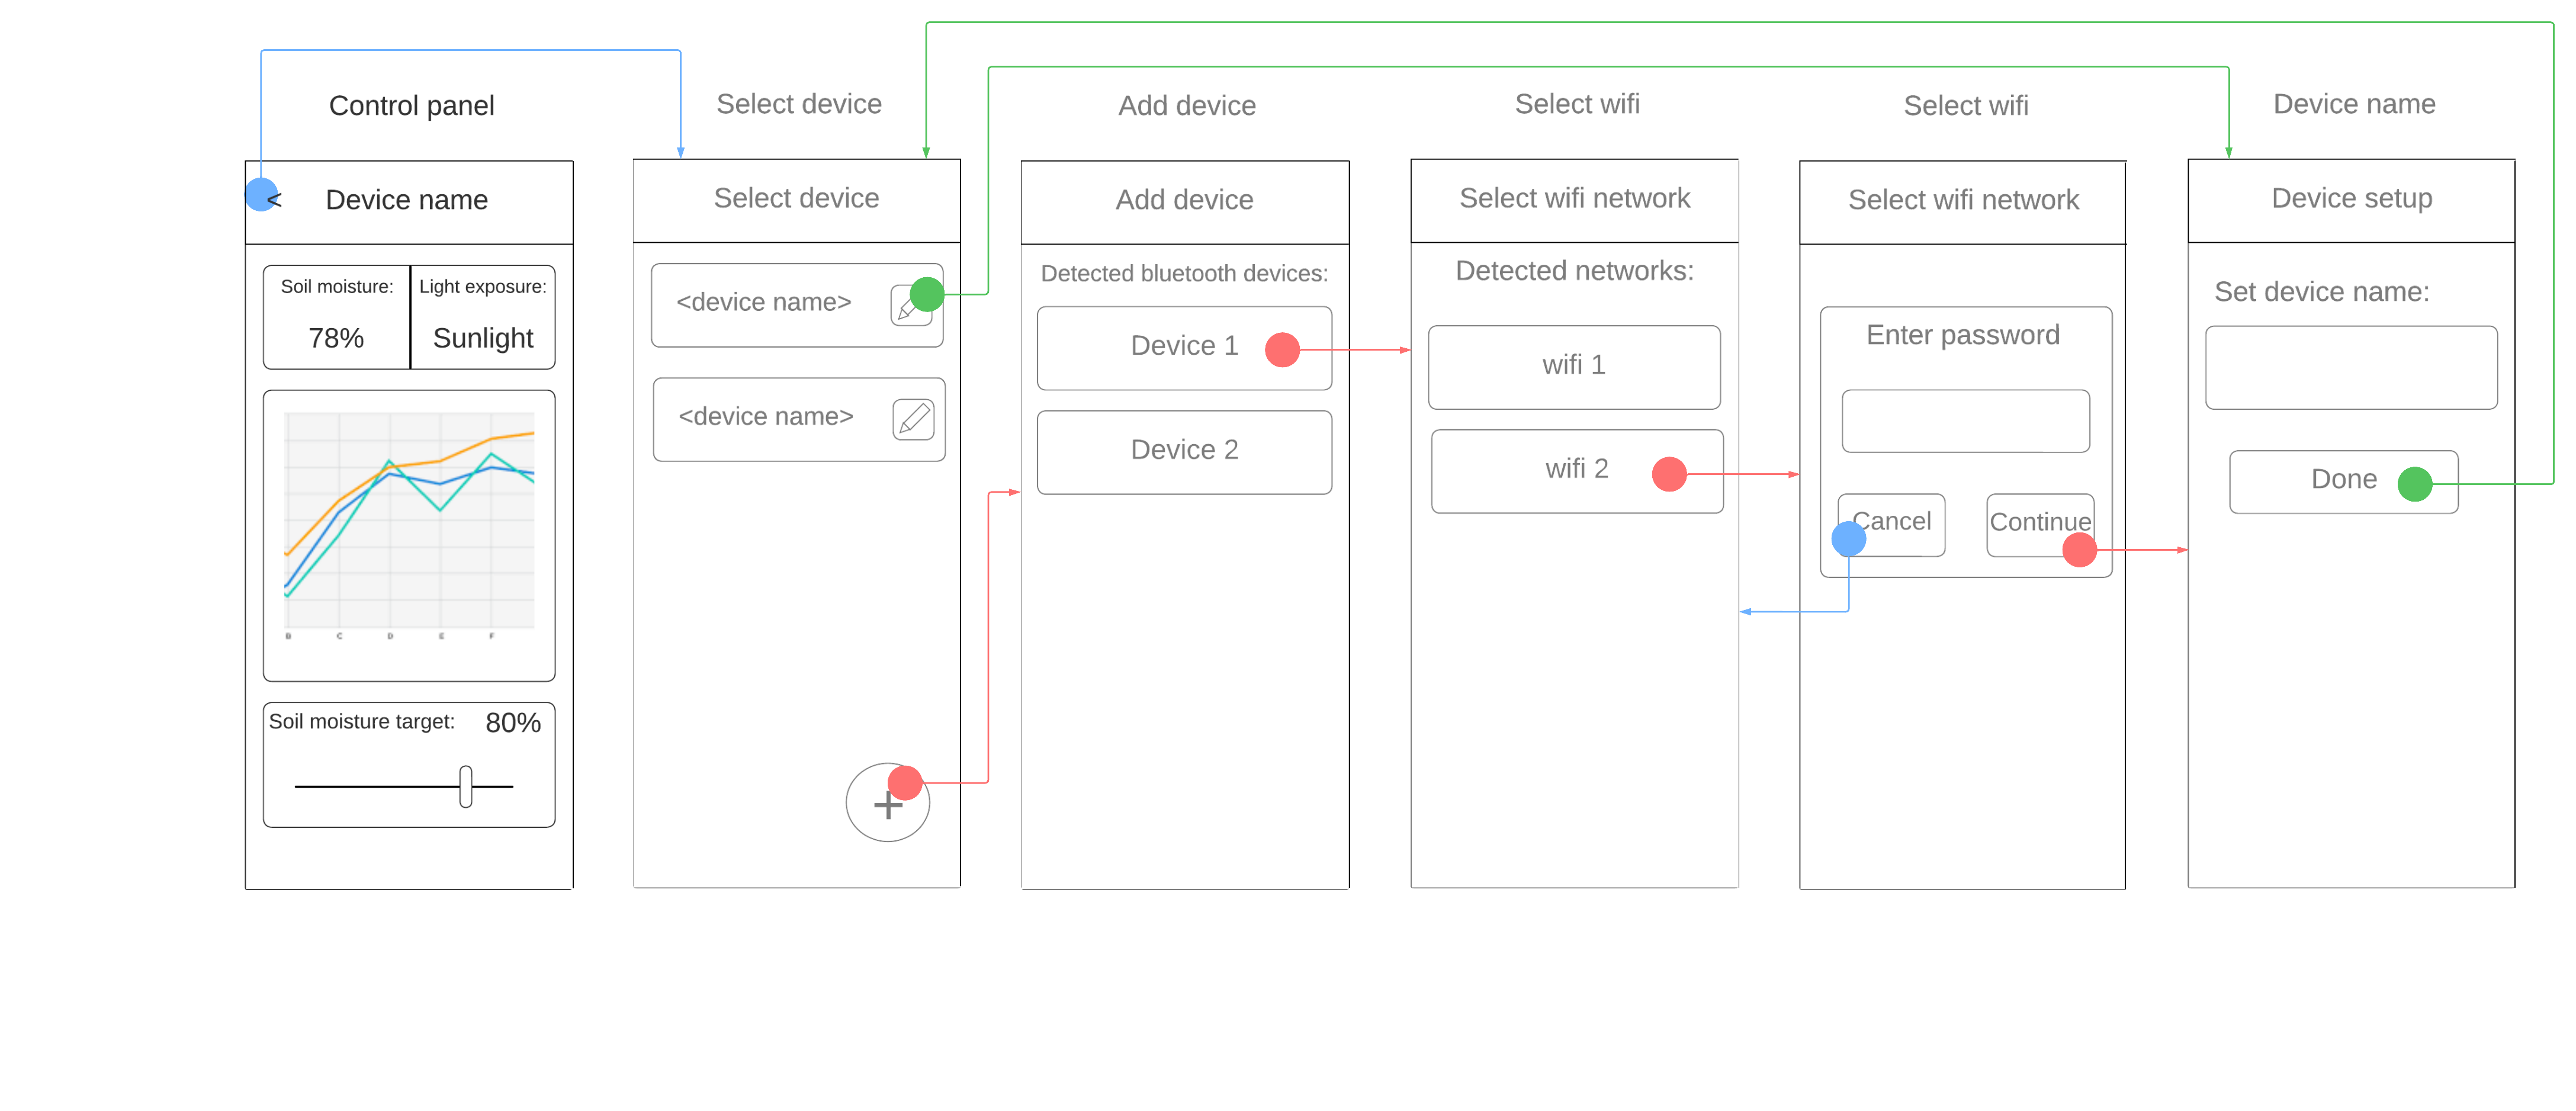
\includegraphics[width= \textwidth]{Report/detail_design/fig/app_flow.png}
    \caption{App flow}
    \label{fig:app_flow}
\end{figure}

\subsection{Connecting to WiFi}
\begin{figure}[!h]
    \centering
    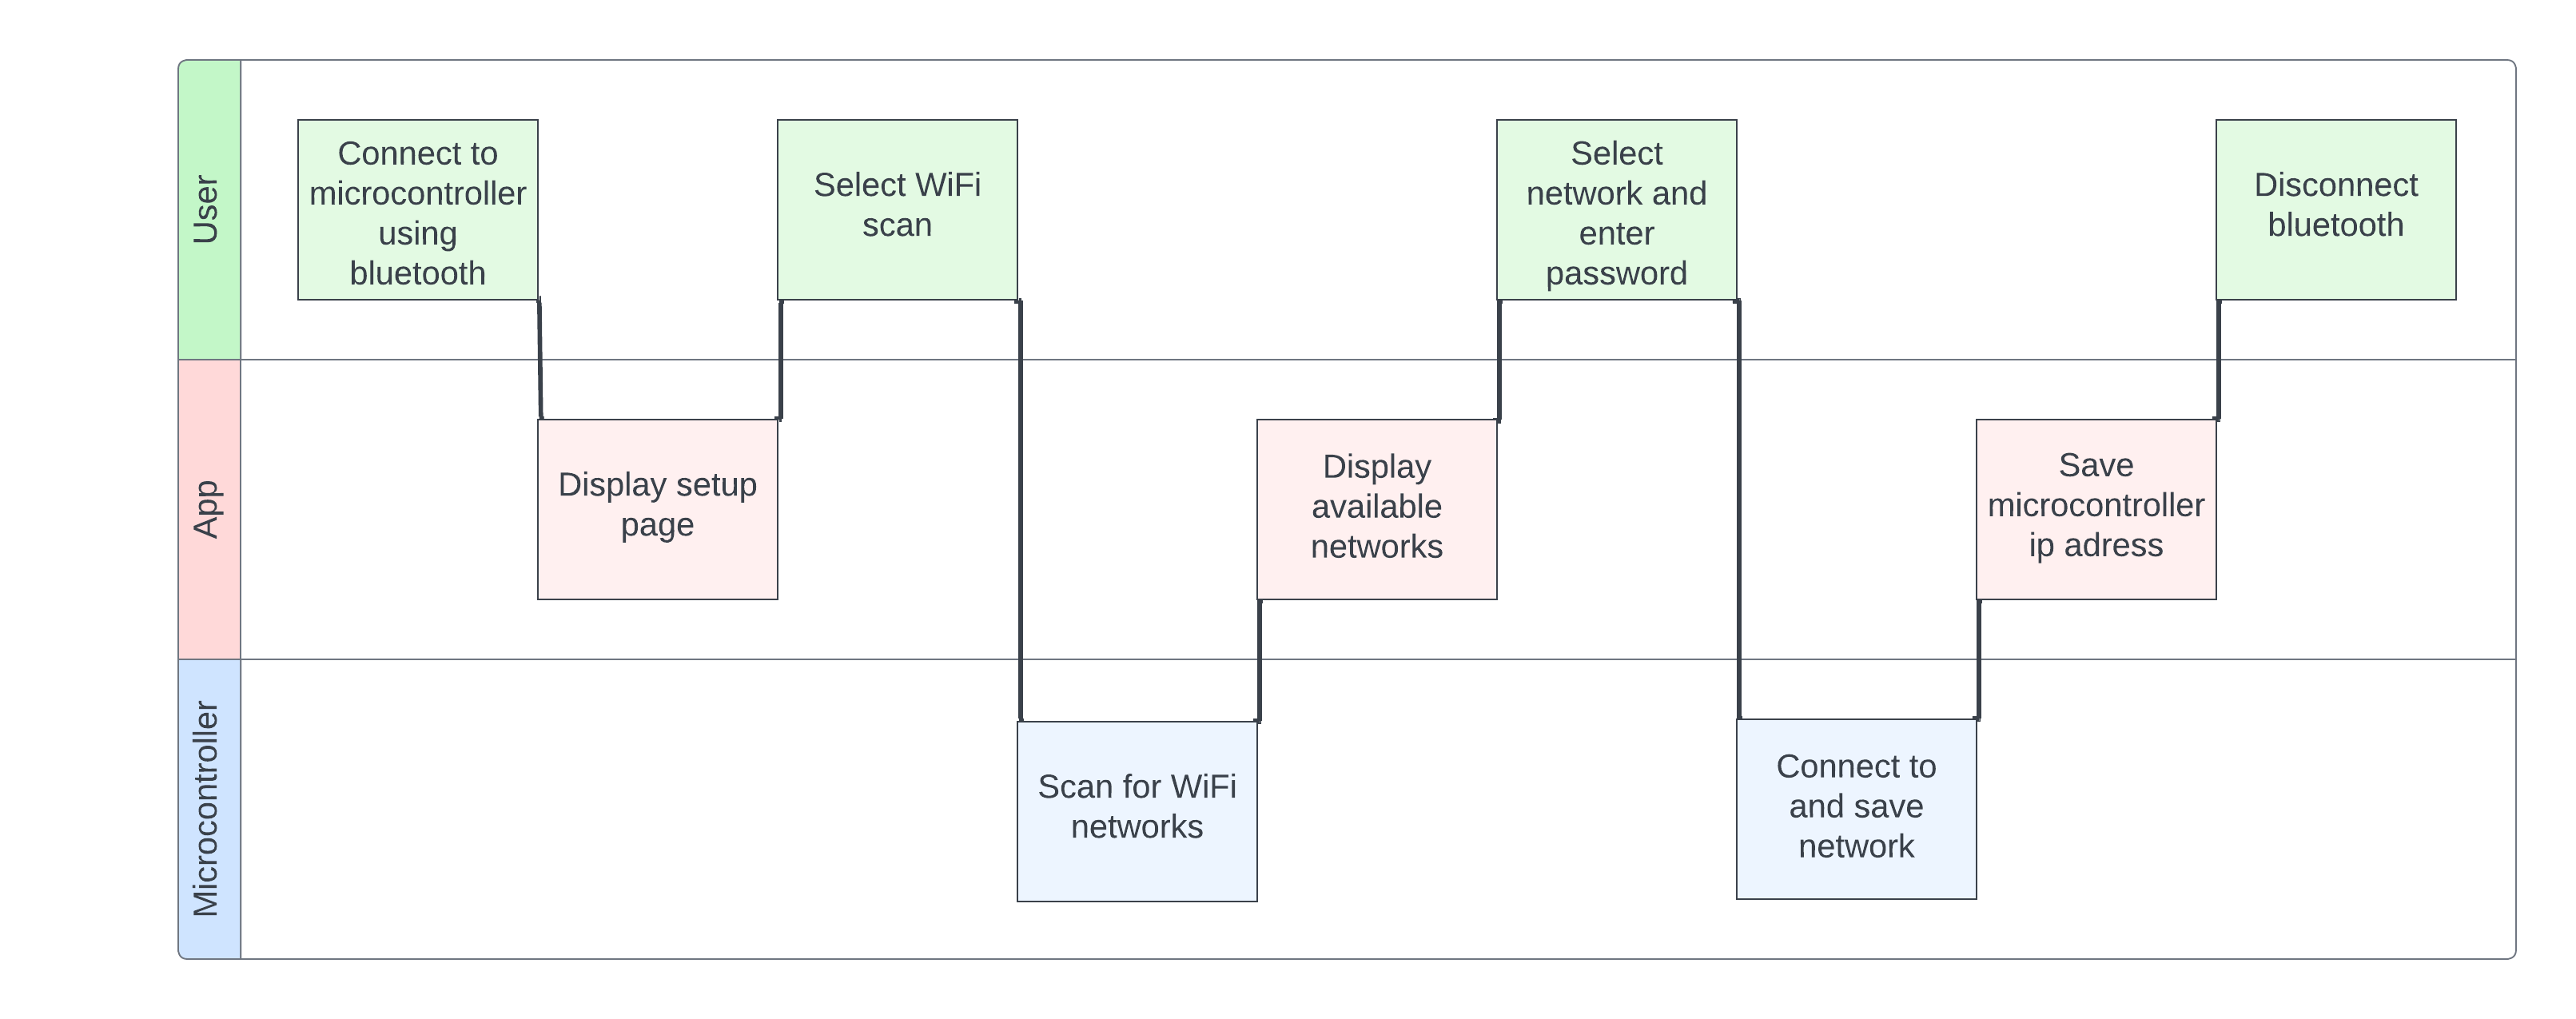
\includegraphics[width= \textwidth]{Report/detail_design/fig/wifi_connect.png}
    \caption{WiFi setup process}
    \label{fig:wifi_setup}
\end{figure}

%%%%%%%%%%%%%%%%%%%%%%%%%%%%%%%%%%%%%%%%
\section{Battery and charging}
\label{sec:battery}
\subsection{battery options}

%%%%%%%%%%%%%%%%%%%%%%%%%%%%%%%%%%%%%%%%
\section{PCB}

%%%%%%%%%%%%%%%%%%%%%%%%%%%%%%%%%%%%%%%%
\section{Case}
